\documentclass[runningheads]{llncs}
%
\usepackage{array}
\usepackage[T1]{fontenc}
\usepackage{placeins}


\usepackage[scaled=0.92]{helvet}

\usepackage[colorlinks=true, linkcolor=blue]{hyperref}

\usepackage[english]{babel}
\selectlanguage{english}

\usepackage{microtype}
\usepackage{graphicx}
\usepackage{wrapfig}
\usepackage{enumitem}
\usepackage{amsmath}
\usepackage{index}
\usepackage[utf8]{inputenc}
\usepackage[svgnames]{xcolor}
\usepackage{url}
\usepackage{hyperref}
\usepackage{float}
\usepackage{longtable}
\usepackage{glossaries}
\usepackage{tabularx}
\usepackage{titletoc}

\begin{document}

\begin{titlepage}

\begin{center}
\vspace*{-1.2in}
\begin{figure}[htb]
\begin{center}

\includegraphics[width=10cm]{Concordia_logo.png}
\end{center}
\end{figure}
\begin{Large}
\vspace*{0.3in}
\textbf{Project Report} \\
\end{Large}
\vspace*{0.1in}
\begin{Large}
For\\
\end{Large}
\vspace*{0.1in}

\begin{Large}
\textbf{Deliverable 2} \\
\end{Large}
\vspace*{0.1in}

\begin{Large}
\textbf{METRICSTICS} \\
\end{Large}
\vspace*{0.3in}

\begin{large}
\textbf{Submitted By} \\
\vspace*{0.1in}
Amrinderpreet Singh\\
Anant Bir Singh\\
Gaganpreet Singh\\
Prabhjot Singh\\
Rahul Singh\\
Piyush Singla\\
\vspace*{0.2in}
\textbf{Submitted to}\\
\vspace*{0.1in}
Prof. Pankaj Kamthan\\
\vspace*{0.3in}

\begin{Large}
\textbf{SOEN 6611 - Software Measurement} \\
\begin{Large}
\vspace*{0.05in}
\textbf{Fall 2023} \\
\end{Large}
\vspace*{0.3in}
\textbf{Concordia University, Montreal, QC}
\end{Large}

\end{large}
\end{center}
\end{titlepage}


\newcommand{\CC}{C\nolinebreak\hspace{-.05em}\raisebox{.4ex}{\tiny\bf +}\nolinebreak\hspace{-.10em}\raisebox{.4ex}{\tiny\bf +}}
\def\CC{{C\nolinebreak[4]\hspace{-.05em}\raisebox{.4ex}{\tiny\bf ++}}}

\setcounter{tocdepth}{2} \tableofcontents
\newpage
\section{Introduction}
This report delves into the creation and evaluation of METRICSTICS,  a comprehensive system designed for the calculation and analysis of various descriptive statistics related to software projects. In this major deliverable, we address key challenges and implement solutions to fulfill the objectives set forth for METRICSTICS.
\subsection{Motivation}
Accurate metrics provide insights into the characteristics and performance of software, aiding in decision-making, resource allocation, and project management. By facilitating the analysis of datasets through measures like mean absolute deviation, standard deviation, and cyclomatic complexity, METRICSTICS equips users with valuable insights into the characteristics and complexities of their software projects. This, in turn, contributes to informed decision-making, efficient project management, and the overall improvement of software quality.
\subsection{Objective}
The primary objective of this report is to document the development and assessment of METRICSTICS. We aim to provide a detailed account of the methodologies employed and outcomes achieved in the course of implementing a software system that addresses various facets of software metrics. Through METRICSTICS, we seek to contribute to the advancement of software measurement practices.

\newpage
\section{PROBLEM 3: Project Effort Estimation}
\subsection{Effort Estimation using Use Case Point (UCP) Approach}
Effort Estimate using use case points is given by:

\[
\text{EffortEstimate} = UCP \cdot PF
\]

where:
\begin{itemize}
    \item $UCP$ is Use Case Points
    \item $PF$ is Productivity Factor
\end{itemize}

$UCP$ is calculated as:

\[
UCP = UUCP \cdot TCF \cdot ECF
\]

where:
\begin{itemize}
    \item $UUCP$ is Unadjusted Use Case Points
    \item $TCF$ is Technical Complexity Factor
    \item $ECF$ is Environmental Complexity Factor
\end{itemize}

$UUCP$ is calculated as:

\[
UUCP = UAW + UUCW
\]

where:
\begin{itemize}
    \item $UAW$ is Unadjusted Actor Weight
    \item $UUCW$ is Unadjusted Use Case Weight
\end{itemize}

Given values:
\begin{align*}
    UAW &= 3 \\
    UUCW &= 10 \\
\end{align*}

\[
UUCP = UAW + UUCW = 3 + 10 = 13
\]
\textbf{Technical Complexity Factor (TCF)}\\
TCF considers technical concerns that can impact the software project. There are 13 different Technical Complexity Factors with their respective weights:

\[
\begin{array}{|c|c|c|}
\hline
\text{TCF Type} & \text{Description} & \text{Weight} \\
\hline
T1 & \text{Distributed System} & 2 \\
T2 & \text{Performance   } & 3 \\
T3 & \text{End User Efficiency   } & 2 \\
T4 & \text{Complex Internal Processing   } & 3 \\
T5 & \text{Reusability} & 1 \\
T6 & \text{Easy to Install} & 0.5 \\
T7 & \text{Easy to Use} & 0.5 \\
T8 & \text{Portability} & 2 \\
T9 & \text{Easy to Change} & 1 \\
T10 & \text{Concurrency} & 1 \\
T11 & \text{Special Security Features} & 1 \\
T12 & \text{Provides Direct Access for Third Parties} & 1 \\
T13 & \text{Special User Training Facilities are Required} & 1 \\
\hline
\end{array}
\]

The values for influence are:
\begin{align*}
    \text{Value of no influence} &= 0 \\
    \text{Value of average influence} &= 3 \\
    \text{Value of strong influence} &= 5 \\
\end{align*}

TCF is calculated as:

\[
TCF = C1 + (C2 \cdot \sum_{i=1}^{13} (WT_i \cdot Fi))
\]

where:
\begin{align*}
    C1 &= 0.6 \\
    C2 &= 0.01 \\
\end{align*}
\begin{equation}
\begin{aligned}
    TCF &= 0.6 + (0.01 \cdot ((2 \cdot 0) + (3 \cdot 3) + (2 \cdot 3) + (3 \cdot 3) + (1 \cdot 5) + (0.5 \cdot 5) \\
    &\quad+ (0.5 \cdot 5) + (2 \cdot 5) + (1 \cdot 5) + (1 \cdot 0) + (1 \cdot 0) + (1 \cdot 0) + (1 \cdot 0))) \\
    &= 0.6 + (0.01 \cdot 64) = 1.24
\end{aligned}
\end{equation}

\textbf{Environmental Complexity Factor (ECF)}\\
ECF accounts for the development team's personal traits and experience. There are 8 Environmental Complexity Factors with their respective weights:

\[
\begin{array}{|c|c|c|}
\hline
\text{ECF Type} & \text{Description} & \text{Weight} \\
\hline
E1 & \text{Familiarity with Use Case Domain} & 1.5 \\
E2 & \text{Part-Time Workers} & -1 \\
E3 & \text{Analyst Capability} & 0.5 \\
E4 & \text{Application Experience} & 0.5 \\
E5 & \text{Object-Oriented Experience} & 1 \\
E6 & \text{Motivation} & 1 \\
E7 & \text{Difficult Programming Language} & -1 \\
E8 & \text{Stable Requirements} & 2 \\
\hline
\end{array}
\]

The values for influence are:
\begin{align*}
    \text{Case: E1, E3, E4, E5, E6, and E8} \\
    &0: \text{No influence} \\
    &1: \text{Strong, Negative influence} \\
    &3: \text{Average influence} \\
    &5: \text{Strong, Positive influence} \\
\end{align*}

\begin{align*}
    \text{Case: E2, E7} \\
    &0: \text{No influence} \\
    &1: \text{Strong, Favorable influence} \\
    &3: \text{Average influence} \\
    &5: \text{Strong, Unfavorable influence} \\
\end{align*}

ECF is calculated as:

\[
ECF = C1 + (C2 \cdot \sum_{i=1}^{8} (WE_i \cdot Fi))
\]

where:
\begin{align*}
    C1 &= 0.14 \\
    C2 &= -0.03 \\
\end{align*}

\[
\begin{aligned}
    ECF &= 1.4 + (-0.03 \cdot ((1.5 \cdot 3) + (-1 \cdot 0) + (0.5 \cdot 5) + (0.5 \cdot 5) \\
    &\quad+ (1 \cdot 5) + (1 \cdot 5) + (-1 \cdot 1) + (2 \cdot 5))) \\
    &= 1.4 + (-0.03 \cdot 28.5) = 0.145
\end{aligned}
\]

\textbf{Calculating UCP and Effort Estimate}\\
Finally, UCP and Effort Estimate are calculated as:

\[
UCP = UUCP \cdot TCF \cdot ECF = 13 \cdot 1.24 \cdot 0.145 = 2.3876
\]

\[
\text{Effort Estimate} = UCP \cdot PF = 2.3876 \cdot 20 = 47.752
\]

\subsection{Effort Estimation using Basic COCOMO 81}

The Basic COCOMO 81 model is used to estimate effort for a software project based on the size of the project in Kilo Lines of Code (KLOC) and its complexity type. The formula for estimating effort is:

\[
\text{Effort (E)} = a \cdot (KLOC)^b
\]

Where:
\begin{itemize}
    \item \(E\) is the effort.
    \item \(KLOC\) is the size of the project in Kilo Lines of Code (1 KLOC = 1000 lines of code).
    \item \(a\) and \(b\) are coefficients that depend on the project type and complexity.
\end{itemize}

The COCOMO 81 model classifies projects into three types:
\begin{enumerate}
    \item Organic: Simple, well-understood projects.
    \item Semi-detached: Intermediate projects with some degree of complexity.
    \item Embedded: Complex, real-time projects.
\end{enumerate}

The values of \(a\) and \(b\) for the organic project type are as follows:

\begin{itemize}
    \item Organic:
    \begin{align*}
        a &= 2.4 \\
        b &= 1.05
    \end{align*}
\end{itemize}

To estimate the effort for our project, you need to determine the size of our project in KLOC and classify it as organic based on its simplicity. Then, use the values of \(a\) and \(b\) to calculate the effort.

For example, if our project is 50 KLOC and you classify it as "organic," you can calculate the effort as follows:

\[ E = 2.4 \cdot (0.542)^{1.05} \]

Now, plug in the values to get the estimated effort:

\[ E = 2.4 \cdot 0.525 \approx 1.262 \]
So, the estimated effort for our project using the Basic COCOMO 81 model is approximately 1.262.

\subsection{Comparison of Estimates and Actual Effort}
In this section, we will compare the effort estimates obtained using the Use Case Point (UCP) approach and the Basic COCOMO 81 model with the actual effort towards the project.\\

\textbf{Estimates using UCP Approach}\\
Using the UCP approach, we estimated the effort required for the project to be approximately 47.752.\\

\textbf{Estimates using Basic COCOMO 81}\\
Using the Basic COCOMO 81 model with the project classified as "organic," we estimated the effort required for the project to be approximately 1.262.\\

\textbf{Actual Effort}\\
Now, let's consider the actual effort that was required to complete the project. After completing the project, the actual effort spent on the project was measured to be around 3 person days.\\

\textbf{Reasons for Variation}\\
There can be several reasons for the variation between the estimated effort and the actual effort for a software project. Some of the common reasons which we think are:

\begin{itemize}
    \item \textbf {Team Experience:} The experience and expertise of the development team can significantly impact the actual effort required. A more experienced team may complete the project more efficiently.
    \item\textbf {Scope Changes:} Changes in project requirements or scope during development can lead to variations in effort. Additional features or modifications can increase effort.
    \item \textbf {Technology Challenges:} Unforeseen technical challenges or issues can arise during development, requiring additional effort to resolve.
    \item\textbf{Project Management:} Effective project management and communication can mitigate variations, while poor management can lead to increased effort.
    \item \textbf{External Factors:} External factors such as market changes, regulatory requirements, or unexpected events can impact project timelines and effort.
\end{itemize}

It's essential to regularly monitor and adapt project plans to address these variations and ensure successful project completion.

\section{PROBLEM 4: Implementation of METRICSTICS}
We have implemented METRICSTICS using object-orientation as the programming paradigm and Python as the programming language. The corresponding code is accessible via our GitHub link.\\
\\
You can access the GitHub repository at:\\
\href{https://github.com/theOGCodeWitcher/SOEN-6611-METRICSTICS}{https://github.com/theOGCodeWitcher/SOEN-6611-METRICSTICS}\\
\\
\subsection{Implementation Details and Design Choices}
 Our application provides users with two choices: they can either upload their own data file or opt to generate random data for metric calculations.
\begin{itemize}
\item \textbf{Programming Style:} The overall structure of the code adheres to \textbf{PEP 8} style guide recommendations
\item\textbf{Modularity:} The code is organized into multiple files (main.py, data\textunderscore processor.py, and helper.py), each serving a specific purpose. The main functionality is encapsulated within the DataProcessor class and the use of helper methods within the Helper class  further supports modularity by separating distinct functionalities.
\item \textbf{Internal Reuse} The generate\textunderscore random\textunderscore data method in the Helper class is reusable for generating random data, promoting a modular and reusable approach.
\end{itemize}

\subsection{Algorithm Selection and Rationale}
We have used the Merge sort, a "divide and conquer" algorithm that efficiently handles the sorting of data by breaking the input into smaller segments, sorting each segment independently, and then merging them back together.\\
\\
\textbf{Rationale for selection}\\
\begin{itemize}
\item Merge sort has a consistent time complexity of O(n log n) in the worst case. This performance is reliable and efficient, regardless of the specific distribution or characteristics of the input data. For a fixed size of 1000 elements, this performance remains reasonable.
\item Merge sort has a straightforward and modular implementation. The divide-and-conquer approach makes the algorithm easier to understand, maintain, and modify. This is beneficial for code readability and future development efforts.
\end{itemize}
\section{PROBLEM 5: Cyclomatic Complexity}
Cyclomatic complexity is a measure of the number of linearly independent paths through a program's source code. It provides an indication of the program's complexity and potential difficulty of maintenance.\\
\\
METRICSTICS is organized into three directories: main.py contains the main graphical user interface (GUI) implemented using Tkinter, handling user interactions and displaying descriptive statistics. data\textunderscore processor.py includes the DataProcessor class responsible for processing input data, calculating statistics such as mean, median, mode, and managing file reading or random data generation. The helper.py module houses the Helper class, providing utility functions for reading different file types, performing arithmetic operations, and aiding in sorting algorithms.

\subsection{Calculation}
Radon is a Python library designed for code analysis and complexity measurement. Leveraging its capabilities, we utilized Radon to calculate cyclomatic complexity of METRICSTICS. Fig.1 illustrates the results obtained. The first letter signifies Block type, Blocks are also classified into three types: functions, methods and classes (see Table~\ref{tab1}) followed by block position and name. The last column signifies Cyclomatic number of a block. Every block is ranked from A (best complexity score) to F (worst one). Ranks corresponds to complexity scores as shown in table 2.

%\begin{tabularx}{0.8\textwidth} { 
 % | >{\centering\arraybackslash}X 
 % | >{\centering\arraybackslash}X | }
 %\hline
 %item 11 & item 12 \\
 %\hline
 %item 21  & item 22  \\
%\hline
%\end{tabularx}
\begin{table}[!htp]
\centering % Center the table
\caption{Block representation}\label{tab1} % Caption and label
\begin{tabularx}{0.8\textwidth} { 
  | >{\centering\arraybackslash}X 
  | >{\centering\arraybackslash}X|  }
\hline
{\bfseries Block Type} & {\bfseries Letter} \\
\hline
Function &  {\bfseries F} \\
Method &  {\large\bfseries M} \\
Class &  {\large\bfseries C} \\
\hline
\end{tabularx}

\vspace{40pt}

\caption{Complexity scores and Ranks}\label{tab2} % Caption and label
\begin{tabularx}{1.1\textwidth} { 
  | >{\centering\arraybackslash}p{0.3\textwidth} 
  | >{\centering\arraybackslash}p{0.2\textwidth}
  | >{\centering\arraybackslash}X|  }
\hline
{\bfseries CC Score} & {\bfseries Rank} & {\bfseries Risk}\\
\hline
1 - 5 &  {\bfseries A} & Low - simple block \\
6 - 10 &  {\bfseries B} & Low - well structured and stable block \\
11 -20 &  {\bfseries C} & Moderate - slightly complex block \\
21 - 30 &  {\bfseries D} & More than moderate - more complex block \\
31 - 40 &  {\bfseries E} & High - complex block, alarming \\
41+ &  {\bfseries F} & Very High - error-prone, unstable block \\
\hline
\end{tabularx}
\end{table}

\FloatBarrier

\begin{figure}[htb]
\begin{center}
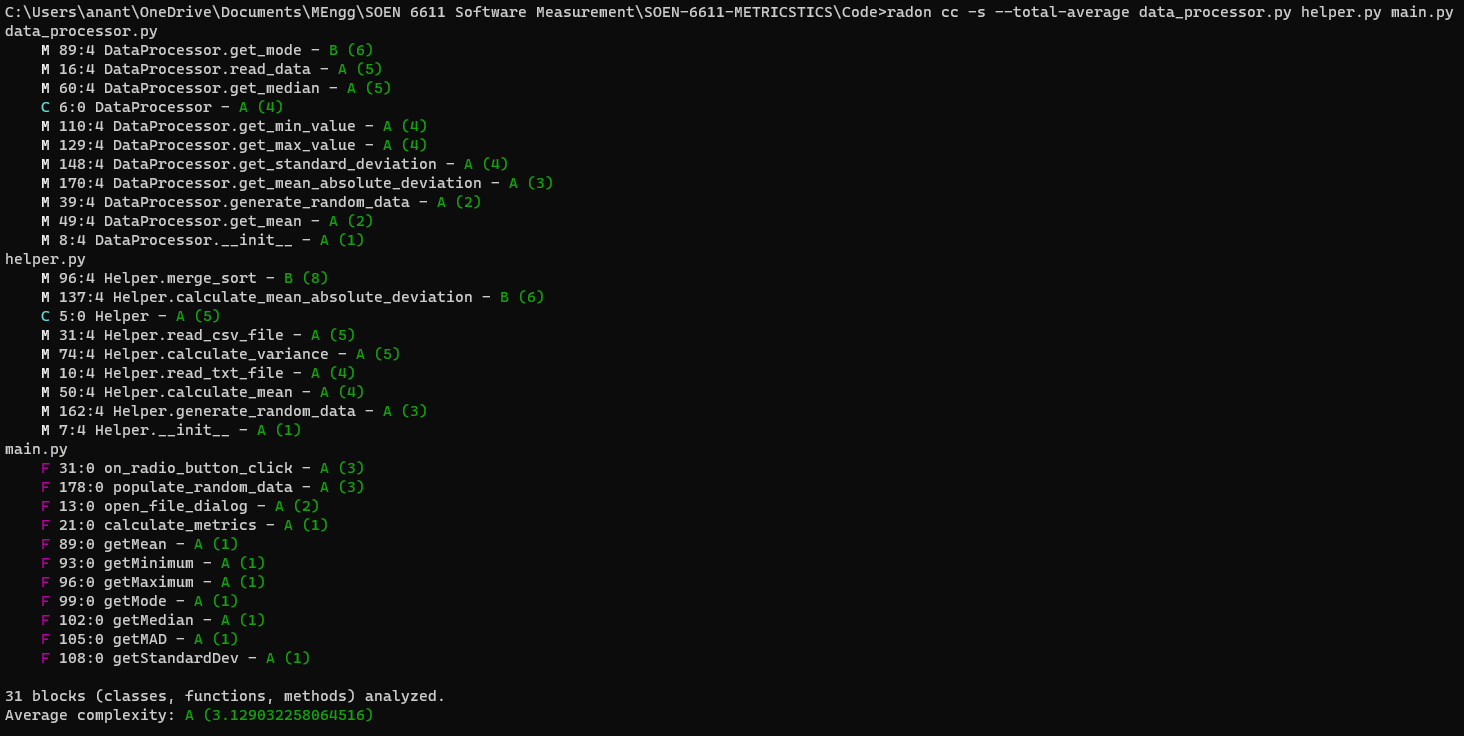
\includegraphics[width=14cm]{Cyclomatic_Complexity.png}
\caption \protect Cyclomatic complexity of various blocks of METRICSTICS
\end{center}
\end{figure}

\vspace{5pt} % Adjust the vertical space as needed

\noindent
The Average Cyclomatic complexity of METRICSTICS is calculated as \textbf{3.129.}

\subsection{Qualitative Conclusions}
\textbf{Average Cyclomatic Complexity:}\\
The average complexity of the functions/methods in METRICSTICS is around 3.13, falling within the low complexity range. This suggests that, on average, the functions/methods are relatively simple and straightforward, promoting maintainability and readability of the codebase.\\
\\
\textbf{Functions/Methods Analysis:}\\
Most of the individual functions/methods have low cyclomatic complexity values, which is generally positive for maintainability and readability. Examining specific functions/methods further supports this observation. For instance, functions like calculate\textunderscore mean, calculate\textunderscore median, and calculate\textunderscore mode demonstrate low individual cyclomatic complexity values, contributing to the overall low average. The simplicity of these functions enhances the codebase's overall comprehensibility and reduces the likelihood of errors during maintenance or future development.

\section{PROBLEM 6: Object-oriented metrics}
The object-oriented metrics, WMC, CF, and LCOM*, for both the classes in METRICSTICS are calculated below.
\subsection{DataProcessor class}
\textbf{Weighted Methods per Class (WMC):}\\
"Weighted Method per Class" (WMC) is a metric used in software engineering to measure the complexity of a class in object-oriented programming. It is a way of quantifying the complexity of a class by assigning weights to different methods based on their characteristics.
\\ \\
The WMC metric is often calculated by summing up the complexity values assigned to each method within a class. The complexity of a method can be assessed based on factors such as the number of control structures (e.g., loops, conditionals), the number of parameters, and other structural attributes.
\\ \\
We already calculated values of complexity for each method in problem 5 so we’ll be directly taking the values from there.

\paragraph{The DataProcessor class has the following methods:}

\begin{enumerate}
    \item \_\_init\_\_ → Complexity : 1
    \item read\_data → Complexity : 5
    \item generate\_random\_data → Complexity : 2
    \item get\_mean → Complexity : 2
    \item get\_median → Complexity : 5
    \item get\_mode → Complexity : 6
    \item get\_min\_value → Complexity : 4
    \item get\_max\_value → Complexity : 4
    \item get\_standard\_deviation → Complexity : 4
    \item get\_mean\_absolute\_deviation → Complexity : 3
\end{enumerate}

\paragraph{WMC = 1 + 5 + 2 + 2 + 5 + 6 + 4 + 4 + 4 + 3 = 36\\ \\}
\textbf{Coupling Factor (CF):}\\
CF measures the interdependence between classes. It can be assessed by examining the dependencies of a class on other classes. In this case, DataProcessor has a dependency on the Helper class.
\\ \\
For DataProcessor, CF = 1 (due to one dependency on Helper).
\\ \\
The coupling factor of 1 indicates that there is a direct dependency on one external class (helper). Lower coupling factors are generally desirable, as they suggest lower interdependence between classes, leading to better modularity and maintainability.\\

\textbf{Lack of Cohesion in Methods (LCOM*):}\\
LCOM* measures the lack of cohesion within a class. It is calculated based on the number of pairs of methods that do not share instance variables.
\\ \\
In this class, there are no attributes (instance variables) explicitly defined. Therefore, the number of attributes accessed (a) is 0. Consequently, the LCOM* formula simplifies to:
\\
LCOM*= m/1
\\ \\
Here, m is the number of methods in the class.
Since there are 9 methods in the DataProcessor class, the LCOM* value would be:
LCOM* = 9/1=9
\\ \\
Therefore, the Lack of Cohesion in Methods (LCOM*) for the DataProcessor class is 9.

\subsection{Helper class}

\textbf{Weighted Methods per Class (WMC):}
\paragraph{The Helper class has the following methods:}

\begin{enumerate}
    \item \_\_init\_\_ → Complexity : 1
    \item read\_txt\_file → Complexity: 4
    \item read\_csv\_file → Complexity: 5
    \item calculate\_mean → Complexity: 4
    \item calculate\_variance → Complexity: 5
    \item merge\_sort→ Complexity: 8
    \item calculate\_mean\_absolute\_deviation → Complexity: 6
    \item generate\_random\_data → Complexity: 3
\end{enumerate}

\paragraph{WMC = 1 + 4 + 5 + 4 + 5 + 8 + 6 + 3 = 36\\ \\}
\textbf{Coupling Factor (CF):}\\
CF for Helper class = 2
\\ \\
In this class, there are two external dependencies:\\ \\
The csv module (imported at the beginning of the file).\\
The random module (imported at the beginning of the file).\\ \\
Therefore, the coupling factor (CF) for helper.py is 2.\\ \\
CF=Number of Dependencies/Number of Classes=2/1=2 \\ \\
The coupling factor of 2 indicates that there are two external dependencies in the Helper class. Lower coupling factors are generally desirable, as they suggest lower interdependence between classes, leading to better modularity and maintainability.\\

\textbf{Lack of Cohesion in Methods (LCOM*):}\\
In this class, there are no attributes (instance variables) explicitly defined. Therefore, the number of attributes accessed (a) is 0. Consequently, the LCOM* formula simplifies to:
\\
LCOM*= m/1
\\ \\
Here, m is the number of methods in the class.
Since there are 7 methods in the Helper class, the LCOM* value would be:
LCOM* = 7/1=7
\\ \\
Therefore, the Lack of Cohesion in Methods (LCOM*) for the Helper class is 7.
\subsection{Qualitative Conclusions}
\textbf{DataProcessor class}\\
Weighted Method Per Class (WMC): 36\\
Conclusion: The class exhibits a high level of complexity with a WMC of 36. Developers should carefully review the methods to identify opportunities for refactoring and simplification.\\ \\
Coupling Factor (CF): 1\\
Conclusion: The class has low coupling with other classes (CF = 1), indicating good encapsulation. This is positive for maintainability and modularity.\\ \\
Lack of Cohesion in Methods (LCOM)*: 9\\
Conclusion: The LCOM* value is moderate, suggesting some room for improvement in terms of method cohesion. Consider restructuring methods for better organization.\\

\textbf{Helper class}\\
Weighted Method Per Class (WMC): 36\\
Conclusion: Similar to data\_processor.py, the class has a high WMC, indicating complexity. Reviewing and potentially refactoring methods may enhance maintainability.\\ \\
Coupling Factor (CF): 2\\
Conclusion:The class exhibits moderate coupling (CF = 2). While not extremely high, developers should be mindful of dependencies to maintain flexibility.\\ \\
Lack of Cohesion in Methods (LCOM)*: 7\\
Conclusion: The LCOM* value is moderate, suggesting some room for improvement in terms of method cohesion. Consider restructuring methods for better organization.

\section{PROBLEM 7: Physical And Logical SLOC}
\subsection{Physical SLOC}
Physical SLOC refers to the number of lines in the source code of a software project that contain executable statements, meaning lines that have actual code instructions and are not blank lines or comments.\\

\textbf{Using Radon}\\
We'll use the Radon library to calculate the physical SLOC. Radon is a Python library that provides various code quality metrics, including physical lines of code. Here's how to use it:\\

\textbf{Installing Radon}\\
We  installed Radon using pip, the Python package manager. Open your terminal and run the following command to install Radon:

\begin{verbatim}
pip install radon
\end{verbatim}

\textbf{Calculating Physical SLOC with Radon}\\
To calculate the physical SLOC using Radon, navigate to the main directory of your project in your terminal and use the following command:

\begin{verbatim}
radon raw main
\end{verbatim}

This command will provide you with a report that includes physical lines of code, as well as other code quality metrics.

\subsection{Logical SLOC}
It is a measure of the size or complexity of a software project based on the number of logical statements or instructions in the source code that affect the program’s control flow or behavior.\\

\textbf{Calculating Logical SLOC with Radon}\\
To calculate the physical SLOC using Radon, navigate to the main directory of your project in your terminal and use the following command:

\begin{verbatim}
radon raw main
\end{verbatim}

\begin{figure}[h]
  \centering
  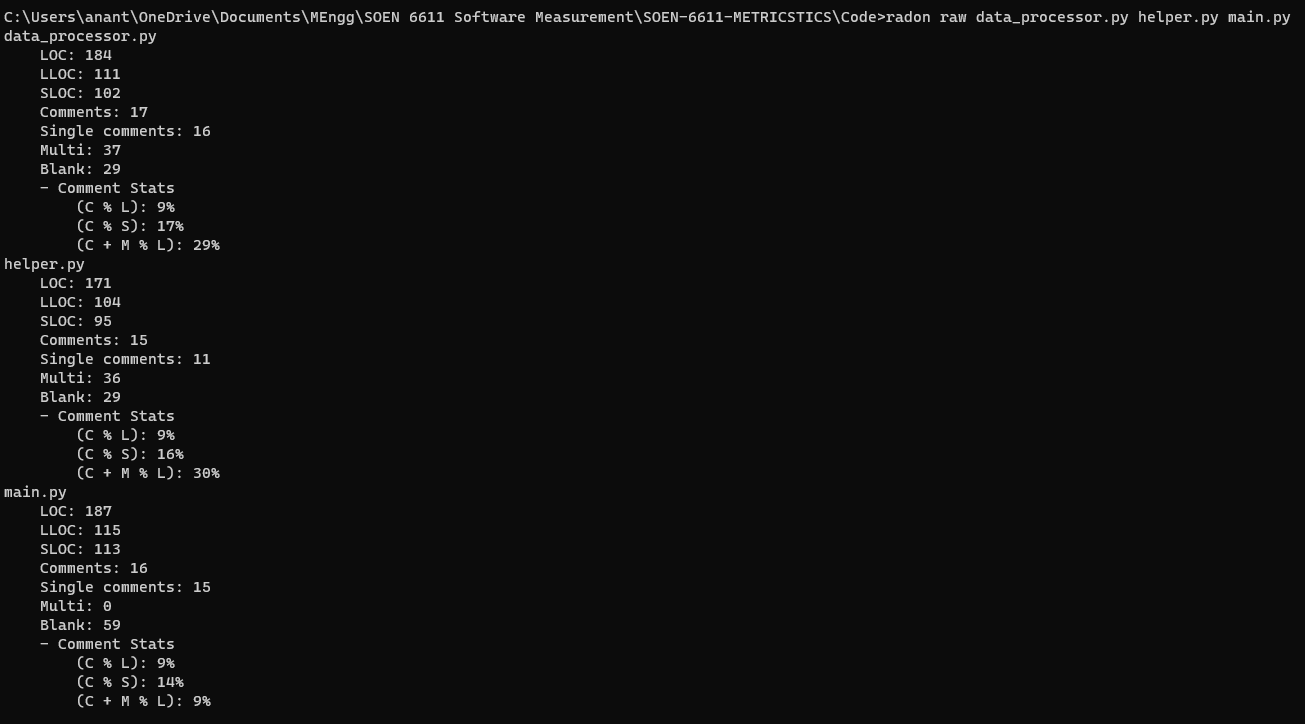
\includegraphics[width=14cm]{LOC.png}
  \caption{Values of Physical and Logical SLOC using Radon}
\end{figure}

\newpage
\subsection{Qualitative Conclusions}
A Logical SLOC of 330, and Physical SLOC of 542  indicate a small size system. It suggests that the software project is small in comparison to generic systems and may have a simpler and
more manageable source code.


\section{PROBLEM 8:WMC vs Logical SLOC}
\subsection{Scatter Plot:}

\begin{table}
\caption{WMC vs Logical SLOC}\label{tab3} % Caption and label
\begin{tabularx}{1.0\textwidth} { 
  | >{\centering\arraybackslash}p{0.5\textwidth} 
  | >{\centering\arraybackslash}p{0.2\textwidth}
  | >{\centering\arraybackslash}X|  }
\hline
{\bfseries Class} & {\bfseries WMC} & {\bfseries Logical SLOC}\\
\hline
DataProcessor&  36 & 111 \\
Helper &  36 &104 \\
\hline
\end{tabularx}
\end{table}

The Weighted Methods per Class (WMC) and Logical Source Lines of Code (Logical SLOC) are both metrics used to measure the complexity or size of a class in software metrics. In general, a higher WMC or Logical SLOC value indicates greater complexity or size. Let's analyze the correlations between these metrics for the provided classes:

\paragraph{DataProcessor:\\}
WMC: 36 \\
Logical SLOC: 111 \\
There is a positive correlation between WMC and Logical SLOC, as both metrics indicate the complexity of the class. In this case, the correlation is moderate, as the WMC is 36 and the Logical SLOC is 111. This suggests that the class has a moderate level of complexity relative to its size.\\ \\

\paragraph{Helper:\\}
WMC: 36 \\
Logical SLOC: 104 \\
Similar to the DataProcessor class, there is a positive correlation between WMC and Logical SLOC. The WMC is 36, and the Logical SLOC is 104, indicating a moderate level of complexity relative to size.\\ \\

\begin{figure}[h]
  \centering
  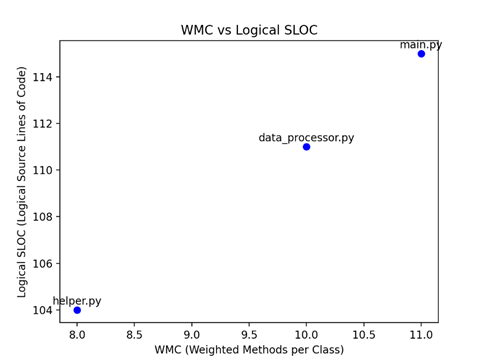
\includegraphics[width=14cm]{SP.png}
  \caption{WMC vs Logical SLOC}
\end{figure}

\newpage
\subsection{Correlation Coefficient}
\text{The scatter plot above indicates that the values of $x$'s and $y$'s are not normally distributed. Consequently, the Spearman's Rank Correlation Coefficient ($r_s$), that is a measure of association for characteristics with non-normally distributed values, can be used to find the correlation coefficient.}

\begin{center}
\begin{tabular}{ |c|c|c|c|c|c|}
\hline
$WMC_{xi}$ & $Rank_{xi}$ & $SLOC$ & $Rank_{yi}$ & $d$ & $d^2$ \\ 
\hline
36 & 2 & 111 & 2 & 0 & 0\\  
\hline
36 & 2 & 104 & 1 & 1 & 1\\
\hline
16 & 1 & 115 & 3 & -2 & 4\\
\hline
\end{tabular}\\
\text{Statistics for calculating $r_s$}
\end{center}

\paragraph{$r_s = 1 - \frac{6\sum_{i=1}^3 D^2} {n( n^2-1 )}$}

\paragraph{$r_s = 1 - \frac{30} {3 \times 8}$}

\paragraph{$r_s = 1-1.25$}

\paragraph{$r_s = -0.25$\\}

\text{The value -0.25 indicates a weak negative correlation.}


\newpage
\section {Conclusion}
In conclusion, this project report provides a comprehensive overview of the development, implementation, and evaluation of a software system aimed at calculating and analyzing various descriptive statistics related to software projects. The report outlines methodologies, and presents outcomes achieved in the course of implementing METRICSTICS.Through thorough documentation and analysis, the report enhances our understanding of software measurement practices, offering a valuable resource for both practitioners and researchers in the field.
\section{Glossary}
\begin{enumerate}
\item \textbf{Scatter Plot:} A type of plot that displays individual data points on a two-dimensional graph. It is used to visualize the relationship between two continuous variables.
\item \textbf{Spearman's Rank Correlation Coefficient ($r_s$):} A measure of statistical dependence between the rankings of two variables. It assesses how well the relationship between two variables can be described using a monotonic function.
\item \textbf{Correlation Coefficient:} A numerical measure that quantifies the strength and direction of a linear relationship between two variables. The correlation coefficient ranges from -1 to 1, where -1 indicates a perfect negative correlation, 1 indicates a perfect positive correlation, and 0 indicates no correlation.
\item \textbf{Monotonic Function:} A function that preserves or reverses the order of elements in its domain. In the context of Spearman's rank correlation, it measures the strength and direction of a monotonic relationship between two variables.
\item \textbf{Weak Negative Correlation:} A correlation between two variables where an increase in one variable tends to be associated with a decrease in the other, but the relationship is not strong.
\end{enumerate}
\begin{thebibliography}{8}
\bibitem{ref_article1}
Pankaj Kamthan, CONTROL FLOW STRUCTURE OF SOURCE CODE.

\bibitem{ref_article2}
Pankaj Kamthan, INTRODUCTION TO SOFTWARE PROJECT COST ESTIMATION.

\bibitem{ref_url1}
\textit{Chatgpt.} ChatGPT. (n.d.).) , \url{https://openai.com/chatgpt.html}

\bibitem{ref_url2}
\textit{Command-line usage\P.} Command-line Usage - Radon 4.1.0 documentation. (n.d.), \url{https://radon.readthedocs.io/en/latest/commandline.html}
\end{thebibliography}


\end{document}
